\section{Theoretischer Hintergrund des Versuches}
\label{sec:Theorie}
\subsection{Halbleiter}
\label{sec:Halbleiter}
Die elektronischen Energiezustände in einem Kristall können durch das Bändermodell beschrieben werden. Nach diesem sind Elektronen in quasikontinuierliche
Bänder gefüllt, zwischen welchen Lücken liegen. In diesen können sich keine Elektronen aufhalten. Das energetisch niedrigere Valenzband ist dabei vollständig 
mit Elektronen gefüllt, während das darüberliegende Leitungsband freie Zustände für Elektronen besitzt. Diese Bandstruktur erklärt die elektrischen Eigenschafen
des jeweiligen Kristalls. Unterschieden werden die leitenden Metalle, in denen die Fermienergie $\epsilon_F$ der Elektronen innerhalb eines Bandes liegt,
die nicht-leitenden Isolatoren, in denen sich keine freien Ladungsträger in dem Leitungsband befinden, und Halbleiter, wo anders als bei den Isolatoren
Elektronen durch Anregung in das Leitungsband gelangen können. 
%Je nach Temperatur und Breite der Bandlücke können Iolatoren und Halbleiter in einander über gehen. 
\begin{figure}[H]
    \centering
    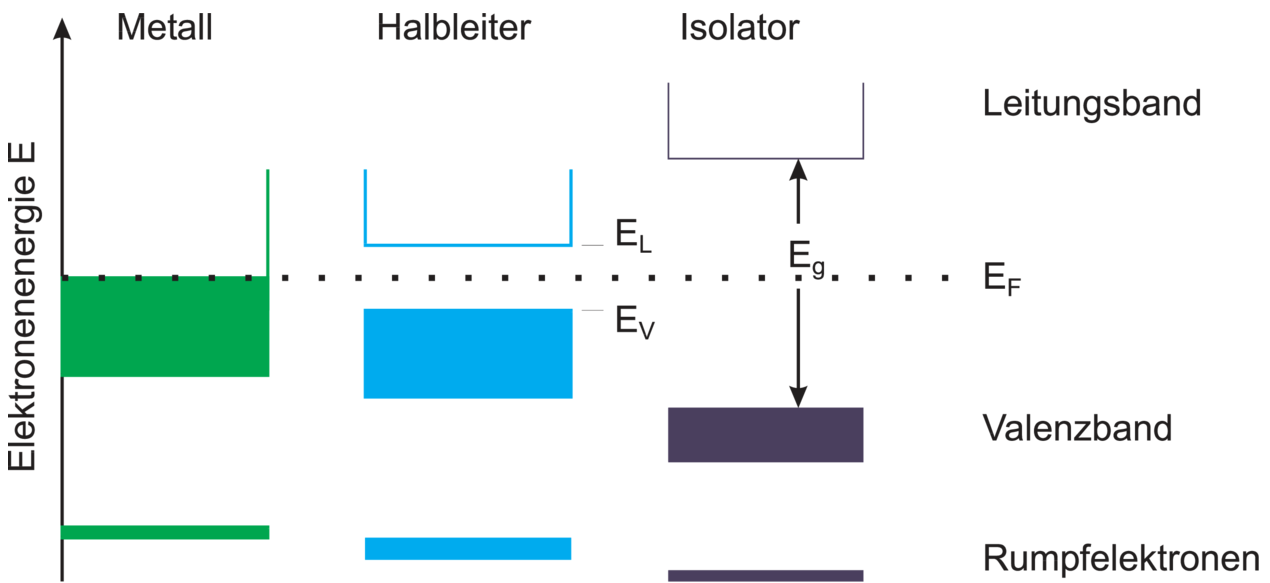
\includegraphics[scale=0.4]{pictures/Bandstrukturen.png}
    \caption{Schematische Bandstrukturen von Metall, Halbleiter und Isolator. \cite{Halbleiter-Grundlagen}}
\end{figure}
\noindent
Gelangt bei einem Halbleiter ein Elektron in das Leitungsband, entsteht durch das fehlende Elektron ein Loch in dem Valenzband, sodass zwei freie 
Ladungsträger entstehen. Zusätzlich zur thermischen Anregungen können bei Halbleitern durch Dotierung auch gezielt Ladungsträger eingebracht werden.
Dabei wird zwischen der n- und p-Dotierung unterschieden. Bei der n-Dotierung werden Donatoratome in den Halbleiter eingebracht, die ein Valenzelektron mehr
besitzen als das Halbleitermaterial. Das Überschusselektron wird dann, wie in Abbildung \ref{fig:Donatorenergie} dargestellt, durch thermische Anregung in das
Leitungsband gehoben. Analog kann bei der p-Dotierung durch Einbringen eines Akzeptors ein Loch erzeugt werden. 
\begin{figure}[H]
    \centering
    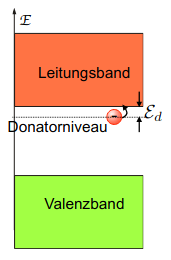
\includegraphics[scale=0.8]{pictures/Donatorelektron.png}
    \caption{Energie des Überschusselektrons in der Bandstruktur. \cite{Halbleiter}}
    \label{fig:Donatorenergie}
\end{figure}
\noindent
Die Leitungselektronen wechselwirken mit dem Kristallpotential, sind also keine freien Teilchen. Als Maß für diese Wechselwirkung wird im Folgenden die 
effektive Masse $m^*$ definiert. Die Elektronenenergie $\epsilon(\vec{k})$ wird für kleine Wellenvektoren $\vec{k}$ zu
\begin{equation}
    \epsilon(\vec{k})=\epsilon(0)+\frac{1}{2}\sum_{i=1}^3\left(\frac{\partial \epsilon^2}{\partial k_i^2}\right)+O(k^4) 
    \label{eqn:Taylor}
\end{equation}
entwickelt. Dieser Ausdruck unterscheidet sich von der Energie eines freien Elektrons
\begin{equation*}
    \epsilon_\text{V=0}=\frac{\hbar^2 k^2}{2m}
\end{equation*}
gerade durch die effektive Masse
\begin{equation*}
    m_i^*=\frac{\hbar²}{\left(\frac{\partial \epsilon^2}{\partial k_i^2}\right)_{k=0}} .
\end{equation*}

\subsection{Zirkulare Doppelbrechung}
\label{sec:Doppelbrechung}
Jede linear polarisierte Welle kann gemäß
\begin{equation}
    E(z)=\frac{1}{2}(E_R(z)+E_L(z))
    \label{eqn:E}   
\end{equation}
als Superposition zweier entgegengesetzt, zirkular polarisierten Wellen dargestellt werden. Dabei gilt
\begin{equation*}
    E_{L/R}=(E_0\vec{x}_0\pm iE_0\vec{y})e^{ik_{L/R}z} .
\end{equation*}
Bei einem optisch aktiven Medium unterscheiden sich aufgrund der Materialstruktur die Phasengeschwindigkeiten der beiden Anteile.
Nachdem die Welle durch einen Kristall der Länge $z=L$ gedrungen ist, lässt sich diese nach Gleichung \ref{eqn:E} beschreiben durch
\begin{equation*}
    E(L)=E_0e^{i\Psi}(\cos{(\theta\vec{x}_0)}+\sin{(\theta\vec{y}_0)})
\end{equation*}
mit den Definitionen
\begin{align*}
    \Psi  &\coloneqq \frac{L}{2}(k_R+k_L)\\
    \theta&\coloneqq \frac{L}{2}(k_R-k_L) .
\end{align*}
Die Polarisationsebene wurde demnach um den Winkel $\theta$ bezüglich der Ausgangslage $\vec{x}_0$ verdreht. Durch geeignete 
Ersetzungen kann $\theta$ auch durch 
\begin{equation*}
    \theta=\frac{L\omega}{2c}(n_R-n_L)
\end{equation*}
ausgedrückt werden, wobei $n$ den Brechungsindex und $\omega$ die Kreisfrequenz der Welle angibt. Die Drehung der Polarisationsebene
um den Winkel $\theta$ ist in Abbildung \ref{fig:Doppelbrechung} visualisiert.
\begin{figure}[H]
    \centering
    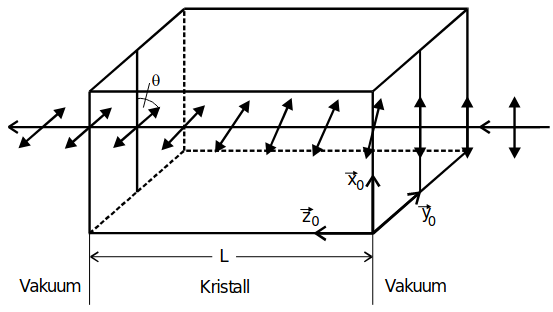
\includegraphics[scale=0.6]{pictures/Doppelbrechung.png}
    \caption{Drehung der Polarisationsebene einer linear polarisierten Welle beim Durchgang durch einen optisch aktiven Kristall. \cite{Anhang}}
    \label{fig:Doppelbrechung}
\end{figure}
\noindent
Mikroskopisch lässt sich die zirkulare Doppelbrechung durch elektrische Dipole verstehen, die in dem Material durch das 
Magentfeld induziert werden. Die makroskopische Polarisation des Kristalls 
\begin{equation*}
    \vec{P}=\epsilon_0\chi\vec{E}
\end{equation*}
ist abhängig von der dielektrischen Suszeptibilität des Stoffes. Es lässt sich zeigen, dass ein Material doppelbrechend ist, wenn
\begin{equation}
    \chi=
    \left[
        \begin{array}{ccc}
        \chi_{xx}          & +i\chi_{xy} & 0         \\ 
        -i\chi_{xy}   & \chi_{yy}        & 0         \\
        0                  & 0                & \chi_{zz}
    \end{array}
    \right]
    \label{eqn:chi}
\end{equation}
gilt. Ist die Suszeptibilität hingegen eine Diagonalmatrix ohne komplexe Einträge, tritt keine Doppelbrechung auf. Ein solches 
Material wird als optisch isotrop bezeichnet. 

\subsection{Der Faraday-Effekt}
Durch Anlegen eines Magnetfeldes kann ein optisch isotropes Material doppelbrechend werden. Es lässt sich für ein gebundenes Elektron in einem 
Magnetfeld die Bewegungsgleichung
\begin{equation*}
    m\ddot{\vec{r}}+K\vec{r}=-e_0\vec{E}-e_0\dot{\vec{r}}\times\vec{B}
\end{equation*}
mit der Kopplungskonstante $K$ des Elektrons an das Kristallfeld aufstellen. 
Da die elektromagnetische Welle mit der Frequenz $\omega$ oszilliert, ist auch die Zeitabhängigkeit des Ortsvektors durch 
\begin{equation*}
    r(t)\propto e^{-i\omega t}
\end{equation*}
gegeben, sodass sich die Bewegungsgleichung zu 
\begin{align*}
    &-m\omega^2\vec{r}+K\vec{r}=-e\vec{E}+ie_0\omega\vec{r}\times\vec{B}\\
    \Leftrightarrow &-\omega^2\vec{P}+K\vec{P}=e_0^2N\vec{E}+ie_0\omega\vec{P}\times\vec{B}
\end{align*}
mit der Polarisation $\vec{P}= -Ne_0\vec{r}$ vereinfacht. Im Rahmen des Versuches gilt für das Magnetfeld $\vec{B}=B\cdot\vec{\text{e}}_\text{z}$. 
Daraus ergibt sich
\begin{equation*}
    \vec{P}=\frac{Ne_0^2}{-m\omega^2+K}\left(\vec{E}+ie_o\omega B
    \left[
    \begin{array}{c}
        P_\text{y}\\
        P_\text{x}\\
        0
    \end{array}
    \right]\right)
    =\epsilon_0\chi\vec{E} .
\end{equation*}
Unter der Bedingung, dass die Einträge $\chi_\text{nm}$ unabhängig von den Komponenten $E_\text{x}$ und $E_\text{y}$ sein sollen, existiert nur eine 
nicht triviale Lösung, wenn $\chi_{B\neq 0}$ die Form \ref{eqn:chi} besitzt. Daraus folgt nach Kapitel \ref{sec:Doppelbrechung}, dass das Material in 
Anwesenheit des Magnetfeldes doppelbrechend geworden ist.

\noindent
Das Matrixelement $\chi_{xy}$ ist gegeben durch 
\begin{equation*}
    \chi_{xy}=\frac{Ne_0^3\omega B}{\epsilon_0(-m\omega^2+K)^2-(e_0\omega B)^2)} .
\end{equation*}
Es ist also insbesondere $\chi_{xy}\neq 0$ für $B\neq 0$. Die Drehung der Polarisationsebene ergibt sich zu 
\begin{equation}
    \theta\approx\frac{L\omega}{2cn}\chi_\text{xy}=\frac{e_0^3}{2\epsilon_0 c m^2}\frac{\omega^2}{(\omega_0^2-\omega^2)^2-\omega_c^2\omega^2}\frac{NBL}{n}
    \label{eqn:theta_kompliziert}
\end{equation}
mit der Zyklotronfrequenz $\omega_c=Be_0/m$ und der Resonanzfrequenz $\omega_0=K/m$. 
%Unter den Annahmen 
%$(\omega_0^2-\omega^2)\gg \omega^2\omega_c^2$ und $\omega_0\gg\omega$vereinfacht sich der Ausdruck \ref{eqn:theta_kompliziert} zu 
%\begin{align}
%    \theta&\approx\frac{e_0^3}{2\epsilon_0 c}\frac{1}{m^2}\frac{\omega^2}{\omega_0^4}\frac{NBL}{n}\\
%    &\frac{2\pi^2e_0^3c}{\epsilon_0}\frac{1}{m^2}\frac{1}{\lambda^2\omega_0^4}\frac{NBL}{n} .
%\end{align}
Für quasifreie Ladungsträger geht $K\to0$ und somit $\omega_0\to 0$. Unter dieser Annahme lässt sich der Ausdruck 
\ref{eqn:theta_kompliziert} zu
\begin{align*}
    \theta&\approx\frac{e_0^3}{2\epsilon_0 c}\frac{1}{m^2}\frac{1}{\omega^2}\frac{NBL}{n}\\
    &=\frac{e_0^3}{8\pi^2\epsilon_0c^3}\frac{1}{m^2}\lambda^2\frac{NBL}{n}
\end{align*} 
nähern. Für Leitungselektronen in einem Kristall entspicht die Masse $m$ nach Kapitel \ref{sec:Halbleiter} der effektiven
Masse $m^*$. Der Zusammenhang zwischen der effektiven Masse eines Leitungselektrons und dem Winkel der Faraday Rotation pro
Länge des Kristalls $\theta_{frei}=\theta/L$ ist demzufolge
\begin{equation}
    \theta_{frei}=\frac{e_0^3}{8\pi^2\epsilon_0c^3}\frac{1}{(m^*)^2}\lambda^2\frac{NBL}{n}.
    \label{eqn:winkel_masse}
\end{equation}
